In this section, we provide the theoretical analysis for fault localization accuracy, communication and storage overhead, and some key parameters. Meanwhile, we analyze the rationalization of \name{}'s source and path verification, bloom filter size and {\tt S}'s detection interval.
\vspace{-0.1in}
\subsection{Fault Localization Accuracy}
\label{localizationaccuracyanalysis}
In this section, we make an in-depth theoretical analysis about fault localization accuracy. In \name{}, no matter what happens in these attacks: source spoofing, forwarding path inconsistency, packet modification and redirection, the packets will be certainly dropped as \name{} enables every entity to perform packet forwarding verification. Therefore, we can regard these abnormal actions as dropping packets.
We respectively define $\theta_{\emph{na}}$ and $\theta_{\emph{mis}}$ as the probability of natural loss and malicious loss (mis-loss) of the entity (as well as its upstream neighbored link), where $\theta_{\emph{mis}} > \theta_{\emph{na}}$.
%We assume there are $m$ packets sent from {\tt S} for one epoch or detection interval.
Thus, the positive ratio threshold $\zeta_\emph{i}$ of $\emph{R}_\emph{i}$ is as Eq. \ref{positiveratiothresholdanalysis} shows, where no malicious loss occurs during packet forwarding.
\begin{equation}\label{positiveratiothresholdanalysis}
\zeta_\emph{i} = 1 - (1 - \theta_{\emph{na}})^i.
\end{equation}
When the misbehaved entity $\emph{R}_\emph{i}$ drops the packets with the probability $\theta_{\emph{mis}}$, its positive ratio $\mathcal{P}_\emph{i}$ is as Eq. \ref{positiveratioanalysis} shows.
\begin{equation}\label{positiveratioanalysis}
\mathcal{P}_\emph{i} = 1 - (1 - \theta_{\emph{na}})^{i-1}\cdot(1 - \theta_{\emph{mis}}).
\end{equation}
Thereby, the fault localization accuracy (denoted by $\delta$) that identifies $\emph{R}_\emph{i}$ as the misbehaved entity is as Eq. \ref{localizationaccuracyanalysis} shows, where P($\cdot$) denotes the probability that satisfies some constraint conditions in brackets. We can learn the higher positive ratio brings about the higher accuracy of fault localization. Based on Eq. \ref{positiveratiothresholdanalysis} and \ref{positiveratioanalysis}, we also learn both the smaller $\theta_{\emph{na}}$ and the larger $\theta_{\emph{mis}}$ contribute to easily localizing the fault.
\begin{equation}\label{localizationaccuracyanalysis}
\delta = P(\mathcal{P}_\emph{i} > \zeta_\emph{i}~\&~\mathcal{P}_1 \leq \zeta_1~\&~\cdots~\&~\mathcal{P}_{\emph{i-}1} \leq \zeta_{\emph{i-}1}).
\end{equation}
\vspace{-0.1in}
\subsection{Communication Overhead}
In \name{} protocol, the \name{} header is the additional communication overhead. From Section \ref{spmoniheaderinitialization}, we can learn (\emph{38+4n}) bytes are occupied in \name{} header, where \emph{n} is the length of $\Psi$. According to the research \cite{huffaker2002distance}, the average end-to-end path length of Internet is 13.11 hops, i.e., \emph{n}=13.11, causing the communication overhead of 90.44 bytes in \name{} protocol.
It is worth mentioning that about 85\% data of Internet is transmitted by large ($>$1400 bytes) packet \cite{portionlargepkt}. 
We can adjust the packet sizes by configuring the interface of Maximum Transmission Unit (MTU). In this case, with packet size $\emph{P}_{\emph{size}}$ = 1500 bytes, \name{} communication overhead accounts for 6.03\% of the entire IP packet.\\
\indent
Compared with other related mechanisms \cite{kim2014lightweight} \cite{cai2015source} \cite{basescu2016high} \cite{naous2011verifying}, \name{} protocol outperforms in terms of communication overhead and its ratio under average path length and large packet (1500 bytes) of Internet, as shown in Table \ref{packetoverheadcom}.
\iffalse
\begin{table}[H]
\scriptsize
\renewcommand\arraystretch{1.5}
\centering
\caption{communication overhead comparison}
\begin{tabular*}{9cm}{llllll}
\toprule
&\emph{\textbf{\name{}}}&\emph{OPT}&\emph{ICING}&\emph{OSV}&\emph{Faultprints}\\
\hline
%general formulation (B) &\textbf{38+4n} & 68+16n & 13+42n & 108+2n&56+8n \\

com-overhead\tnote{1} (Byte)&\textbf{90.44}&277.76&563.62&134.22&160.88\\

com-overhead ratio (\%)&\textbf{6.03\%} & 18.52\% & 37.57\%&8.95\%&10.73\% \\
\bottomrule
\end{tabular*}
\begin{tablenotes}
  \item[1] Com-overhead is short for communication overhead.
\end{tablenotes}
\label{packetoverheadcom}
\end{table}
\fi
%\vspace{-0.1in}
%\iffalse ====================================================
\begin{table}
\caption{Communication Overhead Comparison}
\renewcommand\arraystretch{1.5}%{\multirowsetup}{\centering}
\centerline{
\begin{tabular}{|m{1.8cm}<{\centering}|m{0.7cm}<{\centering}|m{0.7cm}<{\centering}|m{0.7cm}<{\centering}|m{0.7cm}<{\centering}|m{1.2cm}<{\centering}|} %|r|c|l|}%\multirow{5}{2cm}{Source}
%\toprule[2pt]
\hline
\hline
%\cline{1-1}
\centering
&\textbf{RFL} & \textbf{OPT} & \textbf{ICING} & \textbf{OSV} & \textbf{Faultprints}\\\hline \hline
Com-overhead (Byte) & 90.44  & 277.76 & 563.62 & 134.22 & 160.88          \\\hline
Com-overhead ratio (\%) & 6.03  & 18.52 & 37.57 & 8.95 & 10.73          \\\hline
%\bottomrule[2pt]
\hline
\end{tabular}
}
\begin{tablenotes}
  \item[1] Com-overhead is short for communication overhead.
\end{tablenotes}
\label{packetoverheadcom}
\end{table}
%\fi =========================================================
\vspace{-0.1in}
\subsection{Verification Rationalization}
From Section \ref{spmoniheaderinitialization}, we can learn each precomputed marking \emph{M}$_\emph{i}$ occupies 32 bits. The verification at each hop is mainly performed by employing \emph{PRF} to recompute the marking \emph{M}$_\emph{i}$. We must accept that although the inputs are different, there is also the probability, donated by $\varphi$, to result in the same output of \emph{PRF} as the hash collision occurs. As every bit has the equal collision probability (i.e., 0.5), $\varphi$ is the probability that collision of all 32 bits occurs at the same time, i.e., $\varphi$ \emph{=} $\frac{1}{2^{\emph{32}}}$. This illustrates sending 2$^{\emph{32}}$ packets or 2$^{\emph{32}}\cdot\emph{1500}>\emph{2}^{\emph{42}}$=4 TB data (almost impossible for the normal end-to-end communication) will only cause this verification collision, averagely. Therefore, \name{} protocol can perform rationally verification for source authenticity and path compliance as $\varphi$ is small enough.
\vspace{-0.1in}
\subsection{Bloom Filter Size}
In \name{}, end-hosts and intermediate entities all store at least two \emph{bloom filters}, which is an important factor in determining their storage overhead. Although \name{} tries to decrease the storage requirements, blindly reducing \emph{bloom filter} size is not advisable. On one hand, \emph{bloom filter} should be sufficient to store the packet sampling information of one \emph{epoch}, where usage rate $\xi_{\emph{i}}^\emph{e}$ of $\mathcal{B}_{\emph{i}}^e$ does not exceed usage rate threshold $\xi_{\emph{th}}^\emph{e}$. This is also related to the link bandwidth (detailed in Section \ref{monitoringinterval}).
On the other hand, false positive rate increases with the decrease of \emph{bloom filter} size. For one \emph{epoch e}, at most \emph{L}$\cdot\xi_{\emph{th}}^\emph{e}$ packets will be sampled, causing C(\emph{L}, \emph{L}$\cdot\xi_{\emph{th}}^\emph{e}$) sampling results, where C($\cdot$) donates the number of combinations of \emph{L} and \emph{L}$\cdot\xi_{\emph{th}}^\emph{e}$. So the false positive rate is $\mathbb{F}\emph{=}\emph{C}(\emph{L}, ~\emph{L}\cdot\xi_{\emph{th}}^\emph{e})^{\emph{-}1}$.\\
\indent
In this paper, we set \emph{bloom filter} size \emph{L=}1 Kb and usage rate threshold $\xi_{\emph{th}}^\emph{e} \emph{=}$ 0.8. In this case, $\mathbb{F}\ll0.001\%$, which is reasonable in \name{} protocol.
\vspace{-0.1in}
\subsection{Storage Overhead}
\label{storageoverhead}
%\textcolor{red}{We mainly analyze \name{}'s storage overhead for the packet verification and fault localization, while \namekey{}'s storage overhead is described in Section \ref{laskeyevaluation}.}\\
\noindent{\textbf{Router storage overhead.}}
While performing symmetric key distribution, \namekey{} requires intermediate entities to store an established symmetric key (16 bytes) temporarily before its timer expires. Note that \namekey{} is performed only in the initial period of \name{}, and enables each intermediate router to store 16-byte shared key for a short duration\footnote{The duration can be equal to timer threshold, which is evaluated by a round-trip-time (RTT).}. After the shared key is obtained by {\tt S}, each intermediate router don't have to store the symmetric key for per-path or per-source during packet delivery verification. Thus, \name{} provides a lightweight router in terms of the symmetric key storage.\\
\indent 
To sample the forwarded packets, \emph{R}$_\emph{i}$ establishes two \emph{bloom filters} for current and next epoch of each session. Therefore, the storage overhead of router is \emph{2L} bits for per-session and \emph{2NL} bits i.e., O({\tt N}) with the fixed bloom filter size \emph{L} for all sessions, where {\tt N} is the number of sessions in each router per-second. According to the CAIDA results \cite{portionlargepkt}, 12.91K application sessions, on average, are observed in a router per-second. So each router's storage overhead is $\frac{12.91\emph{K}\cdot 2L}{8\cdot1024^2}$ = 3.23 MB for storing bloom filters. 
\begin{figure}%[H]
  % Requires \usepackage{graphicx}
  \centering
  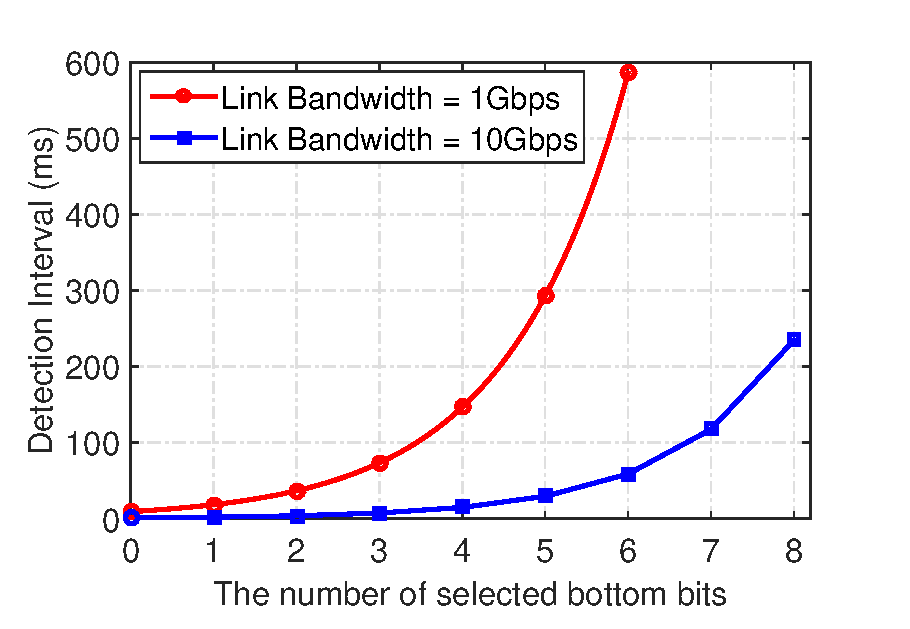
\includegraphics[width=0.65\columnwidth]{code_matlab/tmi2.eps}\\
  \caption{Detection interval $\emph{T}_{\emph{MI}}$ \emph{vs.} the number of selected bottom bits $\omega$.}\label{tmifig}
\end{figure}

\noindent{\textbf{End-host storage overhead.}}
For one session, {\tt S} stores the symmetric keys shared with entities on $\Psi$. With 128 bits length of each secret key, 16(n+1) bytes is occupied to store the keys. 
For each entity, two \emph{bloom filters} are established, resulting in extra storage overhead of 2(n+1)\emph{L} bytes in {\tt S}. So the source storage overhead for one session is (16+2\emph{L})(\emph{n}+1) bytes. On the destination host, only two \emph{bloom filters} should be stored for the packet sampling and localization, introducing its storage overhead of $\frac{2L}{8}$\emph{=}0.25\emph{L} bytes. 
Thus, {\tt S} and {\tt D} have storage overhead of O(n) and O(1) for the fixed bloom filter size \emph{L} per-session. With the average path length of the Internet, their storage overhead is 146.28 bytes and 3.28 bytes, respectively.
\vspace{-0.1in}
\subsection{Detection Interval}
\label{monitoringinterval}
When {\tt S} switches \emph{epoch} value, ReqProb packet is forwarded to all entities on $\Psi$ for requiring their packet sampling information. We respectively define $\emph{T}_{\emph{MI}}$ and $\emph{W}_\emph{B}$ as the detection interval and link bandwidth. As the existence of other sessions, there are at most $\frac{\emph{W}_\emph{B}}{\emph{P}_{\emph{size}}}$ packets of current session and $\frac{\emph{W}_\emph{B}}{2^\omega\cdot\emph{P}_{\emph{size}}}$ packets of each epoch, which can be delivered and sampled by entities per-second. Eq. \ref{tmi} shows the \emph{bloom filter} is consumed to the usage rate threshold $\xi_{\emph{th}}^\emph{e}$ after time interval $\emph{T}_{\emph{MI}}$. 
\begin{equation}\label{tmi}
\begin{split}
\frac{\emph{W}_\emph{B}}{2^\omega\cdot\emph{P}_{\emph{size}}}\cdot\emph{T}_{\emph{MI}} ~\emph{=~ L}\cdot\xi_{\emph{th}}^\emph{e}
~\Rightarrow~\emph{T}_{\emph{MI}} ~\emph{=}~\frac{{L}\cdot\xi_{\emph{th}}^\emph{e}\cdot2^\omega\cdot\emph{P}_{\emph{size}}}{\emph{W}_\emph{B}}
%&\Rightarrow\emph{T}_{\emph{MI}} ~\emph{=}~\frac{9.83\cdot10^6\cdot2^\mathcal{N}}{\emph{W}_\emph{B}}
\end{split}
\end{equation}
When \emph{L=}1 Kb, $\xi_{\emph{th}}^\emph{e}$\emph{=}80\%, \emph{P}$_{\emph{size}}$=1500 bytes and \emph{W}$_\emph{B}$ \emph{=}1 Gbps, we can learn $\emph{T}_{\emph{MI}}$ increases as $\mathcal{N}$ increases at the link bandwidth of both 1 Gbps and 10 Gbps, % ~\emph{=}~$9.375$\cdot2^\mathcal{N}$
as Fig. \ref{tmifig} shows. According to \cite{basescu2016high} \cite{tmi}, with the average value of 225 \emph{ms}, \emph{T}$_{\emph{MI}}$ between 100 \emph{ms} and 350 \emph{ms} conforms to the realistic network. In this case, $\omega$ \emph{=} 5, $\emph{T}_{\emph{MI}}$ \emph{=} 292.97 \emph{ms} when \emph{W}$_\emph{B}$ \emph{=}1 Gbps and $\omega$ \emph{=} 8, $\emph{T}_{\emph{MI}}$ \emph{=} 234.38 \emph{ms} when \emph{W}$_\emph{B}$ \emph{=}10 Gbps meet the requirements of detection interval in realistic network, respectively. 